\documentclass[12pt]{article}
\usepackage{tikz}
\usepackage{amsmath}
\usepackage{amssymb}
\usepackage{amsthm}
\usepackage{bm}
\usepackage{tcolorbox}
\tcbuselibrary{skins}
\usepackage{lipsum}

\usepackage{listings}

%%
%% Julia definition (c) 2014 Jubobs
%%
\lstdefinelanguage{Julia}%
  {morekeywords={abstract,break,case,catch,const,continue,do,else,elseif,%
      end,export,false,for,function,immutable,import,importall,if,in,%
      macro,module,otherwise,quote,return,switch,true,try,type,typealias,%
      using,while},%
   sensitive=true,%
   alsoother={\$},%
   morecomment=[l]\#,%
   morecomment=[n]{\#=}{=\#},%
   morestring=[s]{"}{"},%
   morestring=[m]{'}{'},%
}[keywords,comments,strings]%

\lstset{%
    language         = Julia,
    basicstyle       = \ttfamily,
    keywordstyle     = \bfseries\color{blue},
    stringstyle      = \color{magenta},
    commentstyle     = \color{ForestGreen},
    showstringspaces = false,
}

\usepackage[linesnumbered]{algorithm2e}
\makeatletter
\renewcommand{\@algocf@capt@plain}{above}
\makeatother
\usetikzlibrary{decorations.pathreplacing}
\usetikzlibrary{arrows}
\usetikzlibrary{snakes}
\usetikzlibrary{calc}
\let\emptyset\varnothing
\definecolor{hotpink}{rgb}{0.9,0,0.5}
\definecolor{deepgray}{gray}{0.35}
\definecolor{deepgray2}{gray}{0.25}
\definecolor{deepgray3}{gray}{0.10}
\definecolor{lightgray}{gray}{0.95}
\definecolor{lightgray2}{gray}{0.85}
\definecolor{purple1}{RGB}{239,229,244}
\definecolor{purple2}{RGB}{216,191,216}
\definecolor{lightblue}{rgb}{0.73,0.33,0.83}
\definecolor{lightpurple}{rgb}{.8,.2,.8}
\definecolor{textcolor}{rgb}{0,0,5}
\definecolor{blue1}{RGB}{187,217,238}
\definecolor{blue2}{RGB}{235,244,250}
\definecolor{yellow1}{RGB}{255,255,102}
\definecolor{blue3}{RGB}{63,40,96}
\definecolor{red1}{RGB}{255, 102, 102}
\definecolor{green1}{RGB}{102, 255, 102}
\newtheorem{lemma}{Lemma}
\newtheorem{theorem}{Theorem}
\newtheorem{definition}{Definition}
\theoremstyle{definition}
\def\proof{\par{\bf Proof}. \ignorespaces}
\def\qedsymbol{\vbox{\hrule\hbox{%
                     \vrule height1.3ex\hskip0.8ex\vrule}\hrule}}
\def\endproof{\qquad\qedsymbol\medskip\par}

% \usepackage{booktabs} % For formal tables
% \usepackage{cite}
\usepackage{url}
% \newtheorem{definition}{Definition}[section]
% \newtheorem{theorem}{Theorem}[section]
% \usepackage{algorithmic}
% \usepackage[cmex10]{amsmath}
\usepackage{amssymb}

\title{A Closer Look at Network Flow on Evolving Graphs}

\author{Jiahao Chen \thanks{
Capital One,
New York, USA.
\texttt{cjiahao@gmail.com}
}
 and
Weijian Zhang
\thanks{%
  School of Mathematics,
The University of Manchester,
                Manchester, M13 9PL, England.
\texttt{weijian.zhang@manchester.ac.uk}.
}
}

\def\R{\mathbb{R}}
\def\C{\mathbb{C}}
\def\nbyn{n \times n}
\def\mbyn{m \times n}
\def\l{\lambda}
\def\norm#1{\|#1\|}
\def\normi#1{\|#1\|_1}
\def\normo#1{\|#1\|_{\infty}}
\def\Chat{\widehat{C}}
\def\e{eigenvalue}

% \DeclareMathOperator{\diag}{diag}   % Requires amsmath.
\def\diag{\mathop{\mathrm{diag}}}     % If not using amsmath.
\def\trace{\mathop{\mathrm{trace}}}   % If not using amsmath.

\def\At{\widetilde{A}}
\def\normt#1{\|#1\|_2}

% Note: this clashes with amsmath.
\def\bmatrix#1{\left[\matrix{#1}\right]}

\newenvironment{njh}{\begin{quote}\small\sf{\color{blue}$\diamondsuit$~NJH~}}{\end{quote}}
\newenvironment{wz}{\begin{quote}\small\sf{\color{green}$\diamondsuit$~WZ~}}{\end{quote}}

\begin{document}

%\subtitlenote{The full version of the author's guide is available as
 % \texttt{acmart.pdf} document}


\maketitle

\begin{abstract}
This paper studies the influence of the temporal information in an evolving graph on the node centrality scores.
In particular, we look at four important centrality measures, namely Katz centrality,
Resolvent Betweenness centrality, Closeness centrality, and PageRank.

We derive evolving graph centrality measures from the perspective of network flow and
observe that the amount of temporal distance between nodes has an important impact on the final evolving graph centrality scores, especially on the top ranked nodes.
Build on this idea, we introduce a generalised PageRank on evolving graph that is based on two ideas:
reverse network flow and block adjacency matrix.
We conduct our experiments on random evolving graphs and the JMLR co-author networks to illustrate our idea.
\end{abstract}

\section{Introduction}
\label{sec:introduction}

In the 1985 science-fiction film ``Back to the Future'', Marty McFly (played by Michael J. Fox) travelled back in time and accidentally changed history.
However, we cannot travel back in time or even send a message to the past.
To traverse an evolving graph, a.k.a a time-dependent graph, one has to consider order of time stamps. In particular, a walk on an evolving graph needs to be time-preserving, meaning we
can not pass a massage (through an edge) to a node at a earlier time.
Time-preversing walks and paths are very important concepts for
network flow on evolving graphs.

% time-respecting walk
We represent an evolving graph as a time-ordered sequences of graphs, similar to the work of Tang and coworkers \cite{nicosia13, tang09, tang102, tang10} and Grindrod, Higham and coworkers \cite{grindrod13,grindrod11}. The idea is to divide the system's time span into temporal slices and regards it as a sequence of static graphs $G^{[t]}$, one for each layer. Such representation arises naturally in many real-world applications. For example,
consider networks of users interacting through messaging. Each interaction between two users $A$ and $B$ are stored with a time stamp $t$. If we represent a user as a node then a user $A$ at time stamp $t$ is represented by a pair $(v,t)$ and a message sent from user $A$ to user $B$ at time stamp $t$ can be represented as $\langle (A, t) (B, t) \rangle$.

In general, a node $v$ on $G^{[t]}$ is represented by a pair $(v, t)$, where $t$ is the time stamp of the graph $G^{[t]}$.
A sequence of interactions between users form a walk. Suppose $A$ sent a message to $B$ at time stamp $t_1$
and then $B$ sent this message to $C$ at time stamp $t_2$. We can represent this activity as $\langle (A,t_1), (B,t_1), (B, t_2), (C,t_2)\rangle$, where each pair of two nodes has meanings: $\langle (A,t_1), (B,t_1) \rangle$ and $\langle (B,t_2), (C,t_2) \rangle$ represent interactions between users $A$, $B$, and $C$ and $\langle (B,t_1), (B,t_2) \rangle$ represents the fact that user $B$ holds the message at time stamp $t_1$ and $t_2$.

A time-respecting walk is a sequence of nodes $\langle (v_1, t_1), (v_2, t_2), \ldots ,(v_m, t_m)\rangle$, where $t_1 \le t_2 \le \cdots \le t_n$ are the corresponding time stamps. If $t_i = t_j$, then $\langle (v_i, t_i), (v_j, t_j) \rangle$ is an edge where both nodes are on the same temporal slice,  otherwise it is an edge linking nodes from different temporal slices.
We call edges of the first kind \emph{static edges} and of the second kind \emph{causal edges}.
Recall in static graph, a walk of length $m$ is defined as a sequence of nodes $v_1, v_2, \ldots, v_{m+1}$ such that for each $i = 1, \ldots, m$ there is an edge from $v_i$ to $v_{i+1}$. How to determine the length of a time-respecting walk?
One could define the length of a time-respecting walk as the total number of temporal slices (see shortest temporal distance in \cite{tang09}) or the number of static edges (see dynamic walk in \cite{grindrod11}). This paper studies the impact of these two different definitions. In particular, we studies a general definition of temporal distance that takes account of both temporal slices and static edges.


% Related works
Researchers have generalised many static graph centrality algorithms for evolving graphs. One approach is to use the fact that the elements of the matrix product of adjacency matrices at different time stamps can correctly count the number of temporal paths.
However, not every centrality algorithm can be generalised in this way. Another approach is to define evolving graph centrality algorithms using time-respecting paths. This approach is applicable to algorithms that are defined using shortest paths.


% no work on pagerank so far. By understanding temporal walk, we could provide a generalization of pagerank on evolving graphs.

% In Higham's following up papers, time delay is considered as alternative format of Katz centrality.
% But the impact of temporal is left unconsidered. We studied the problem on centrality from two different types of centrality: one that depends on matrix unfolding and one that depends on temporal walk.


% our contribution this paper
Borgatti \cite{borgatti05} noted that the manner of traffic flow entails a new way to think about centrality. In particularly, the importance of a node in a network can not be determined without reference to how traffic flows through the network.
Inspired by this idea, we simulate network flows in evolving graphs to measure the centrality scores.
% Grindrod et al.'s definition of dynamic walk \cite{grindrod11} only counts static edges.
% Tang et al. \cite{tang10s} measure a temporal shortest walk in time unit (or causal edges) only.
% If a node can be reached by another node in $k$ time stamps then the distance between the two nodes is $k$. Chen and Zhang \cite{chen16} considered both static edges and causal edges in their definition of temporal walk.
The aims of this paper are as follows. First, to derive important evolving graph centrality from first principle via network flow. Second, to study the impact of temporal distance between nodes on centrality.
Third, to generalise PageRank on evolving graphs.
We carry out the experiment using the Julia dynamic network analysis package
EvolvingGraphs.jl (\url{https://github.com/EtymoIO/EvolvingGraphs.jl}).
We use the research paper data gathered from Etymo (\url{https://etymo.io}), a visual search engine for data scientists.


\section{Motivation: A Closer Look at Katz Centrality on Evolving Graphs}
\label{sec:motivation}

We let $G_n = \langle G^{[1]}, G^{[2]}, \ldots, G^{[n]} \rangle$ be an evolving graph
and $A^{[1]}, A^{[2]}, \dots A^{[n]}$ be the corresponding adjacency matrices.
Then the dynamic communicability matrix is defined as
\begin{equation}
  \label{eq:q}
  Q^{[k]} = (I - \alpha A^{[1]})^{-1}(I - \alpha A^{[2]})^{-1} \cdots (I -  \alpha A^{[n]})^{-1},
\end{equation}
where parameter $\alpha < 1/ \max_k \rho(A^{[k]})$, the spectral radius of $A^{[k]}$.
The $i$th row sum of $Q^{[k]}$ is the broadcast centrality.


Suppose $A$, $B$, and $C$ are three co-workers in a large internet company. Figure \ref{fig:katz_eg}
shows how they exchange ideas during $3$ days at work. The directions of the arrows indicate the direction of the flow of ideas.
For example, $A$ shares a new idea with $B$ on day $1$ and $B$ shares a new idea with $C$ on dat $3$. As a result, $A$'s idea can influence $C$.

\begin{figure}[h]
 \begin{center}
    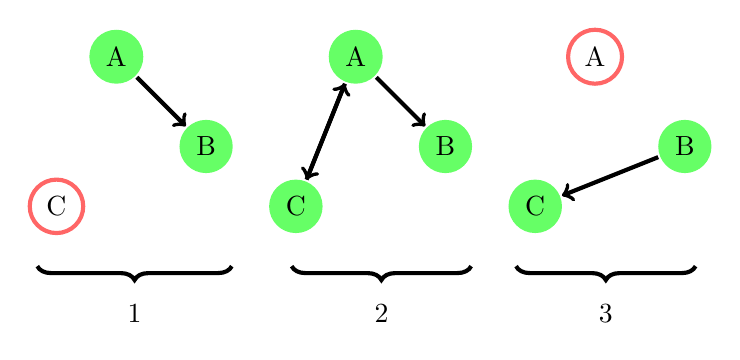
\begin{tikzpicture}[scale=.38, line width =1.5pt]
  \node[circle,fill=green1, minimum size=0.2cm] (n7) at (-5,7) {B};
  \node[circle,draw=red1, minimum size=0.2cm] (n8) at (-10,5) {C};
  \node[circle,fill=green1, minimum size=0.2cm] (n10) at (-8,10) {A};
  \node[circle,fill=green1, minimum size=0.2cm] (n6) at (3,7) {B};
  \node[circle,fill=green1, minimum size=0.2cm] (n4) at (-2,5) {C};
  \node[circle,fill=green1, minimum size=0.2cm] (n1) at (0,10) {A};
   \node[circle,fill=green1, minimum size=0.2cm] (n11) at (11,7) {B};
  \node[circle,fill=green1, minimum size=0.2cm] (n12) at (6,5)  {C};
  \node[circle,draw=red1, minimum size=0.2cm] (n14) at (8,10) {A};
  \foreach \from/\to in {n10/n7, n1/n4, n4/n1, n11/n12, n1/n6}
   \draw[every edge,->] (\from) -- (\to);
 %\draw[dotted,->](n4) -- (n12);
% \draw[dotted,->](n7) to[out=80, in=40](n11);
\draw [decorate,decoration={brace,amplitude=5pt},xshift=-4pt,yshift=0pt]
(-4,3) -- (-10.5,3) node [midway,yshift=-0.6cm]{ $1$};
\draw [decorate,decoration={brace,amplitude=5pt},xshift=-4pt,yshift=0pt]
(4,3) -- (-2,3) node [midway,yshift=-0.6cm]{$2$};
\draw [decorate,decoration={brace,amplitude=5pt},xshift=-4pt,yshift=0pt]
(11.5,3) -- (5.5,3) node [midway,yshift=-0.6cm]{ $3$};
    \end{tikzpicture}
\end{center}
\caption{An evolving directed graph with 3 time stamps $1$, $2$ and $3$.
At each time stamp, the evolving graph is represented as a graph.
The green filled circles represent active nodes while the red circles represent
inactive nodes. Directed edges in each time stamp are shown as black arrows.}
\label{fig:katz_eg}
\end{figure}

We could use EvolvingGraphs.jl to generate the above evolving graph and compute the Katz centrality.

\begin{lstlisting}
using EvolvingGraphs
using EvolvingGraphs.Centrality

g = EvolvingGraph{Node{String}, Int}()
add_bunch_of_edges!(g, [("A", "B", 1), ("A", "C", 2),
("A", "B", 2),("C", "A", 2),("B", "C", 3)])
\end{lstlisting}

The centrality values for each node are
\begin{lstlisting}
katz(g)
3-element Array{Tuple{EvolvingGraphs.Node{String},Float64},1}:
 (Node(A), 0.742301)
 (Node(B), 0.42943)
 (Node(C), 0.514373)
\end{lstlisting}

As expected $A$ is the most important node in the network. $C$ is the second important node in the network as it influenced
$A$ at time stamp $2$. If we reverse the time of communication between day $1$ and $3$, i.e., $B$ shares a new idea with $C$ on day $1$ and $A$ shares a new idea with $B$ on day $3$. Then in this case the idea $A$ had on day $3$ can not pass to $C$. This is illustrated in Figure \ref{fig:katz_eg2}.

\begin{figure}[h]
 \begin{center}
    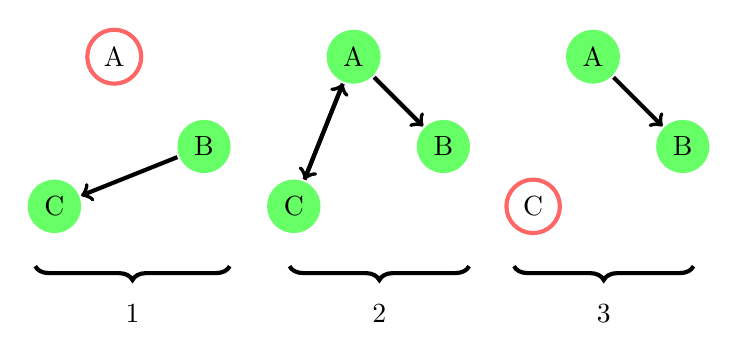
\begin{tikzpicture}[scale=.38, line width =1.5pt]
  \node[circle,fill=green1, minimum size=0.2cm] (n7) at (-5,7) {B};
  \node[circle,fill=green1, minimum size=0.2cm] (n8) at (-10,5) {C};
  \node[circle,draw=red1, minimum size=0.2cm] (n10) at (-8,10) {A};
  \node[circle,fill=green1, minimum size=0.2cm] (n6) at (3,7) {B};
  \node[circle,fill=green1, minimum size=0.2cm] (n4) at (-2,5) {C};
  \node[circle,fill=green1, minimum size=0.2cm] (n1) at (0,10) {A};
   \node[circle,fill=green1, minimum size=0.2cm] (n11) at (11,7) {B};
  \node[circle,draw=red1, minimum size=0.2cm] (n12) at (6,5)  {C};
  \node[circle,fill=green1, minimum size=0.2cm] (n14) at (8,10) {A};
  \foreach \from/\to in {n7/n8, n1/n4, n4/n1, n1/n6, n14/n11}
   \draw[every edge,->] (\from) -- (\to);
 %\draw[dotted,->](n4) -- (n12);
% \draw[dotted,->](n7) to[out=80, in=40](n11);
\draw [decorate,decoration={brace,amplitude=5pt},xshift=-4pt,yshift=0pt]
(-4,3) -- (-10.5,3) node [midway,yshift=-0.6cm]{ $1$};
\draw [decorate,decoration={brace,amplitude=5pt},xshift=-4pt,yshift=0pt]
(4,3) -- (-2,3) node [midway,yshift=-0.6cm]{ $2$};
\draw [decorate,decoration={brace,amplitude=5pt},xshift=-4pt,yshift=0pt]
(11.5,3) -- (5.5,3) node [midway,yshift=-0.6cm]{ $3$};
    \end{tikzpicture}
\end{center}
\caption{An evolving directed graph with 3 time stamps $1$, $2$ and $3$.
At each time stamp, the evolving graph is represented as a graph.
The green filled circles represent active nodes while the red circles represent
inactive nodes. Directed edges in each time stamp are shown as black arrows.}
\label{fig:katz_eg2}
\end{figure}

In this cast, we have
\begin{lstlisting}
g2 = EvolvingGraph{Node{String}, Int}()
add_bunch_of_edges!(g2, [("A", "B", 3), ("A", "C", 2),
("A", "B", 2),("C", "A", 2),("B", "C", 1)])
\end{lstlisting}

The centrality ratings of the three nodes are

\begin{lstlisting}
katz(g2)
3-element Array{Tuple{EvolvingGraphs.Node{String},Float64},1}:
 (Node(A), 0.687679)
 (Node(B), 0.490062)
 (Node(C), 0.535666)
\end{lstlisting}

Notice the rating of $A$ decreased as its influence is not as important as in Figure \ref{fig:katz_eg}.
% does not take account of walks in a long time. cost in time
If the communication between $A$, $B$, and $C$ are not on three consecutive days
but on day $1$, day $10$, and day $100$, as shown in Figure \ref{fig:katz_eg3},
we would expect the centrality scores to change. However, according to \eqref{eq:q}, scores are unchanged.
We notice that the generalised Katz centrality on evolving graphs only takes account of the edges at each time stamp but not the communication time between edges at different time stamps.

\begin{figure}[h]
 \begin{center}
    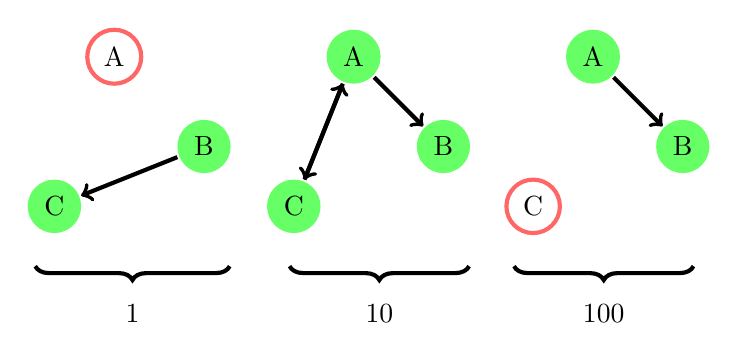
\begin{tikzpicture}[scale=.38, line width =1.5pt]
  \node[circle,fill=green1, minimum size=0.2cm] (n7) at (-5,7) {B};
  \node[circle,fill=green1, minimum size=0.2cm] (n8) at (-10,5) {C};
  \node[circle,draw=red1, minimum size=0.2cm] (n10) at (-8,10) {A};
  \node[circle,fill=green1, minimum size=0.2cm] (n6) at (3,7) {B};
  \node[circle,fill=green1, minimum size=0.2cm] (n4) at (-2,5) {C};
  \node[circle,fill=green1, minimum size=0.2cm] (n1) at (0,10) {A};
   \node[circle,fill=green1, minimum size=0.2cm] (n11) at (11,7) {B};
  \node[circle,draw=red1, minimum size=0.2cm] (n12) at (6,5)  {C};
  \node[circle,fill=green1, minimum size=0.2cm] (n14) at (8,10) {A};
  \foreach \from/\to in {n7/n8, n1/n4, n4/n1, n1/n6, n14/n11}
   \draw[every edge,->] (\from) -- (\to);
 %\draw[dotted,->](n4) -- (n12);
% \draw[dotted,->](n7) to[out=80, in=40](n11);
\draw [decorate,decoration={brace,amplitude=5pt},xshift=-4pt,yshift=0pt]
(-4,3) -- (-10.5,3) node [midway,yshift=-0.6cm]{ $1$};
\draw [decorate,decoration={brace,amplitude=5pt},xshift=-4pt,yshift=0pt]
(4,3) -- (-2,3) node [midway,yshift=-0.6cm]{ $10$};
\draw [decorate,decoration={brace,amplitude=5pt},xshift=-4pt,yshift=0pt]
(11.5,3) -- (5.5,3) node [midway,yshift=-0.6cm]{ $100$};
    \end{tikzpicture}
\end{center}
\caption{An evolving directed graph with 3 time stamps $1$, $10$ and $100$.
At each time stamp, the evolving graph is represented as a graph.
The green filled circles represent active nodes while the red circles represent
inactive nodes. Directed edges in each time stamp are shown as black arrows.}
\label{fig:katz_eg3}
\end{figure}


\section{Time-Preserving Walks and Paths}
\label{sec:time-pres-paths}

% what is walk and what is path?
A walk of length $l$ is a sequence of nodes $v_1, v_2, \ldots, v_l, v_{l+1}$ such that for
each $i = 1, 2, \ldots, l$, there is an edge from $v_i$ to $v_{i+1}$. A path of length $l$ is a walk of length $l$
such that all the nodes are different.
% relate to centrality
The definition of centrality depends on the manner in which traffic flows through a network \cite{borgatti05}.
Time-preserving walks induce temporal Katz centrality and temporal closeness centrality while time-preserving paths induce betweenness centrality and closeness centrality.


We now describe evolving graph network flow in more details. We follow the definition of
\emph{evolving graph} in \cite{chen16}.

\begin{definition}
  An \textbf{evolving graph} $G_n$ is a sequence of (static) graphs
$G_n = \langle G^{[1]}, G^{[2]},  \ldots ,G^{[n]} \rangle$ with associated time stamps
$t_1, t_2, \ldots, t_n$ respectively. Each $G^{[t]} = (V^{[t]}, E^{[t]})$ represents a (static) graph labelled by a time t.
\end{definition}

Note the node sets $V^{[t]}$ can change over time, i.e., nodes may appear or disappear at a particular time stamp.
For example, in Figure \ref{fig:eg_shortest_walk}, at time stamp $1998$, $V^{[1998]} = \langle 1, 2 \rangle$ and $E^{[1998]} = \langle (1,2) \rangle$. Each graph $G^{[t]}$ can be represented by its adjacency matrix $A^{[t]}$.
We can represent $G_n$ by a list of adjacency matrices $A_n = \langle A^{[1]}, A^{[2]}, \ldots, A^{[n]} \rangle$.

If we only measure the temporal difference in a temporal walk, we have a new definition of Katz centrality.
In the matrix form, the nonzero entries of $A^{[t_i]} A^{[t_{i+1}]}$ counts all the temporal walks of length $1$, and
$A^{[t_i]}\cdots A^{[t_j]}$, where $i < j$ counts all the temporal walks of length $j -i$.
For example, $A^{[1]}A^{[4]}$, $A^{[1]}A^{[1]}A^{[4]}$ and $A^{[1]}A^{[2]}A^{[3]}A^{[4]}$ are all walks of length 3.
In the original Katz centrality, the `attenuation' factor $\alpha$ is imposed on the
number of paths, i.e., longer paths has smaller effect to the overall rating.
Hence the final result is the summation of all products of the form
\[
\alpha^k A^{[i]} \cdots A^{[i+k]}
\]
Note this can not be written in \eqref{eq:q} as discussed in Section \ref{sec:temp-katz-centr}.


% Another definition of temporal walk was introduced by \cite{chen16}. Here
% both static edges and causal edges are considered. We can represent an evolving graph by a block adjacency matrix, as shown in Section \ref{sec:centr-block-adjac}. Centrality on this block matrix gives the importance of each node at all time stamps. We can average these rating at different time stamps to
% get the final rating.

\begin{figure}[h]
 \begin{center}
    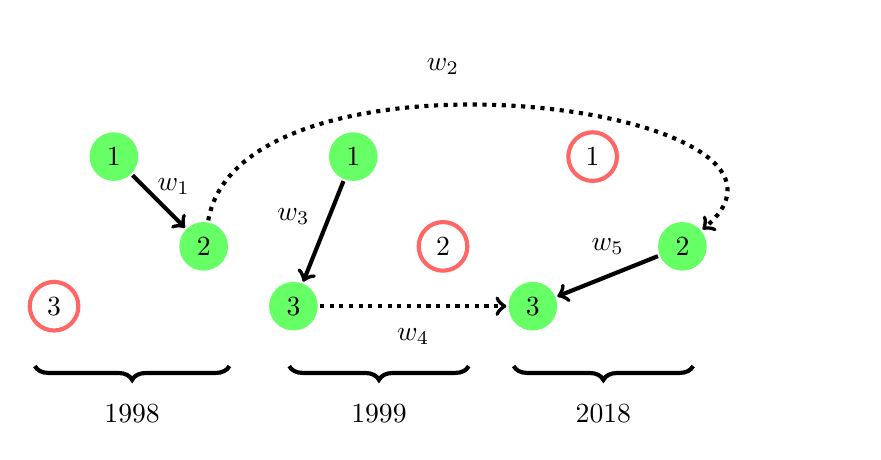
\begin{tikzpicture}[scale=.38, line width =1.5pt]
  \node[circle,fill=green1, minimum size=0.2cm] (n7) at (-5,7) {2};
  \node[circle,draw=red1, minimum size=0.2cm] (n8) at (-10,5) {3};
  \node[circle,fill=green1, minimum size=0.2cm] (n10) at (-8,10) {1};
  \node[circle,draw=red1, minimum size=0.2cm] (n6) at (3,7) {2};
  \node[circle,fill=green1, minimum size=0.2cm] (n4) at (-2,5) {3};
  \node[circle,fill=green1, minimum size=0.2cm] (n1) at (0,10) {1};
   \node[circle,fill=green1, minimum size=0.2cm] (n11) at (11,7) {2};
  \node[circle,fill=green1, minimum size=0.2cm] (n12) at (6,5)  {3};
  \node[circle,draw=red1, minimum size=0.2cm] (n14) at (8,10) {1};
  \node (w1) at (-6, 9) {$w_1$};
  \node (w2) at (3, 13) {$w_2$};
  \node (w3) at (-2, 8) {$w_3$};
  \node (w4) at (2, 4) {$w_4$};
  \node (w5) at (8.5, 7) {$w_5$};s
  \foreach \from/\to in {n10/n7, n1/n4, n11/n12}
   \draw[every edge,->] (\from) -- (\to);
 \draw[dotted,->](n4) -- (n12);
\draw[dotted,->](n7) to[out=80, in=40](n11);
\draw [decorate,decoration={brace,amplitude=5pt},xshift=-4pt,yshift=0pt]
(-4,3) -- (-10.5,3) node [midway,yshift=-0.6cm]{ $1998$};
\draw [decorate,decoration={brace,amplitude=5pt},xshift=-4pt,yshift=0pt]
(4,3) -- (-2,3) node [midway,yshift=-0.6cm]{ $1999$};
\draw [decorate,decoration={brace,amplitude=5pt},xshift=-4pt,yshift=0pt]
(11.5,3) -- (5.5,3) node [midway,yshift=-0.6cm]{ $2018$};
    \end{tikzpicture}
\end{center}
\caption{An evolving directed graph with 3 time stamps $1998$, $1999$ and $2018$.
At each time stamp, the evolving graph is represented as a graph.
The green filled circles represent active nodes while the red circles represent
inactive nodes. Directed edges in each time stamp are shown as black arrows and directed edges between graphs are shown as dotted arrows, where $w_1, w_2 \ldots w_5$ are edge weights.}
\label{fig:eg_shortest_walk}
\end{figure}


\begin{definition}
  A \textbf{temporal node} is a pair (v, t), where $v \in V^{[t]}$ is a node at a time $t$.
\end{definition}

%At each time stamp, we only count temporal nodes that connects by an edge.

\begin{definition}
  A temporal node $(v, t)$ is an \textbf{active node} if there exists at least one edge $e \in E^{[t]}$ that connects $v \in V^{[t]}$ to another node $w \in V^{[t]}, w\ne v$. Otherwise it is called an inactive node.
\end{definition}

In Figure \ref{fig:eg_shortest_walk}, the filled green circles are active nodes. For the adjacency matrix representation, a node $i$ is active at time stamp $t$, then
the $i$th row or the $i$th column of $A^{[t]}$ has at least one none-zero entry.

 \begin{definition}
 A \textbf{static edge} $\langle (v_i, t), (v_j, t)\rangle$ is a pair of elements of $V^{[t]}$, i.e., $v_i \in V^{[t]}$ and
 $v_j \in V^{[t]}$.
  A \textbf{causal edge} $\langle (v, t_i), (v, t_j)\rangle$ is a pair of the same node at different time stamps.
 \end{definition}

 For example, in Figure \ref{fig:eg_shortest_walk}
 $\langle (1, 1998), (2, 1998) \rangle$ is a static edge at time stamp $1998$ and $\langle (3, 1999), (3, 2018) \rangle$ is a causal edge between time stamp $1999$ and time stamp $2018$.
 The difference between static edges and causal edges were first explicitly considered in \cite{chen16}.


 We can denote a \emph{weighted static edge} as $\langle (v_i, t), (v_j, t), w_s \rangle$ and a \emph{weighted causal edge} as $\langle (v, t_i), (v, t_j), w_t \rangle$.
 Here $w_s$ represents the spatial distance between the two nodes $v_i$ and $v_j$; $w_t$ represents the
 temporal distance of $v$ at different time stamps.
 In Figure \ref{fig:eg_shortest_walk}, the black arrows represent static edges and the dotted arrows represent causal edges.
 Suppose we assign all the static edge weight to $1$ and
 let the causal edge weight be the number of time stamps between the pair of nodes. Then in Figure \ref{fig:eg_shortest_walk}
 the edge weight between $(1, 1998)$ and $(2, 1998)$ is $1$ and the edge weight between $(2, 1998)$ and $(2, 2018)$ is $10$.
In general, a time-preserving walk can be defined as follows.


\begin{definition}
A \textbf{time-preserving walk}  of length $m$ on an evolving graph $G_n$ is a time-ordered sequence of active nodes, $\langle (v_1, t_1), (v_2, t_2), \ldots, (v_m, t_m) \rangle$, where $t_1 \le t_2 \le \cdots \le t_m$ and
$v_i = v_j$ if and only if $t_i \ne t_j$.
\end{definition}

It is natural to define the length of a walk on a static graph as the number of nodes travelled through the walk. For the weighted graph case, the length of a walk is the total weight of all the edges in the walk. We observe that static edges link nodes in space while causal edges link nodes in time. Hence we would like to distinguish temporal distance from spatial distance in an evolving graph: we let the length of a static edge be one and the length of a causal edge be the temporal distance between the two nodes. In the simplest case, the time-respecting walk
$\langle (1, 1998) ,(2, 1998) , (2, 2018), (3, 2018)\rangle$ in Figure \ref{fig:eg_shortest_walk} has length $12$ in total because two static edges $\langle (1, 1998) (2, 1998) \rangle$ and $\langle (2, 2018), (3, 2018) \rangle$ each have length one, and $\langle (2, 1998) (2, 2018) \rangle$
traverse $10$ time stamps and thuse has length $10$.

A time-preserving walk (and path) can traverse both causal edges and static edges.
The following Julia function measures the temporal distance between two active nodes in an evolving graph.

\begin{lstlisting}
function temporal_distance(v1::TimeNode,
                           v2::TimeNode, beta::Real = 1.)
  beta* abs(node_timestamp(v1) - node_timestamp(v2))
end
\end{lstlisting}
which means the temporal distance is the difference between their time stamps scaled a hyper-parameter
\texttt{beta}.

\section{Centrality Measures}
\label{sec:topol-temp-flow}

% what is centrality?
Centrality measures the importance of nodes within a graph.
% current evolving graph centrality approach
To generalize centrality measures for evolving graphs there are two common approaches.
First, we could exploit the fact that matrix product of adjacency matrices at different time stamps counts the number of dynamic walks in an evolving graph. Using this idea, we can generalize walk-based centrality measures such as
the Katz Centrality \cite{estrada09} and Communicability Betweenness \cite{alsayed15}.
Second, we could generalize the definition of shortest paths as shortest temporal paths and replace shortest paths in centrality measures with shortest temporal paths where possible. This way we can define temporal betweenness centrality and temporal closeness centrality \cite{nicosia13}.

% our approach
We observe both approaches ignore the communication time between edges at different time stamps, i.e., the time gap between different (static) graph slices. We take account of this communication time by deriving centrality measures from the original theses of the ideas and show communication time has important impact on the final node ratings (and rankings).
We note that our goal is not about providing efficient centrality algorithms which is out of the scope of this paper.

\subsection{Temporal Katz Centrality}
\label{sec:temp-katz-centr}

% katz centrality from first principle
Katz Centrality accounts the influence of nearest-neighbours to a give node and the influence of other nodes
separated at a certain distance from it. The $k$th power of adjacency matrix $A$, i.e., $A^k$, of a graph $G$ accounts for walk of length $k$. The expansion
\begin{equation}
  \label{eq:a}
  A^0 + \alpha A + \alpha^2 A^2 + \cdots,
\end{equation}
converges to $(I - \alpha A)^{-1}$ when $\alpha < 1/\rho(A)$, the spectral radius of $A$. The $(i,j)$ entry of \eqref{eq:a}
accounts all walks from $i$ and $j$ with the influence of walks of length $k$ scaled by a factor of $\alpha^k$.
The Katz centrality of node $i$ is the $i$th row sum of $(I - \alpha A)^{-1}$, which is the sum of influence of all the nodes that node $i$ can reach via a walk.
In other words, we start with node $i$ and each out-neighbour of node $i$ has influence $\alpha$ on node $i$ and the out-neighbour of out-neighbour of node $i$ has influence $\alpha^2$ on node $i$, and so on.

For evolving graphs, we replace out-neighbours with forward neighbours which preserve the direction of time.
Then the Katz score of a node $i$ at time stamp $t$, denoted by $(i,t)$, is the sum of influence of all the active nodes that $(i,t)$ can reach via a time-preserving walk.
Unlike \cite{grindrod11}, we also consider the temporal distance between two nodes. For example, the temporal distance between $(i, 2001)$ and $(i, 2018)$ is $17$.
% julia code implementation
With the definition of \texttt{temporal\_distance} introduced in Section \ref{sec:time-pres-paths}.
We define the temporal Katz score of node $(i, t)$ as

\begin{lstlisting}[caption={Temporal Katz Centrality of Single Node},label={lst:katz}]
function temporal_katz(g::AbstractEvolvingGraph,
  start::TimeNode; alpha = 0.2, max_level = 10)
    score = 0.
    v = start
    fronter = [v]
    level = 0
    while level < max_level
        next = []
        for u in fronter
            for v in forward_neighbors(g, u)
                push!(next, v)
                if node_key(v) != node_key(u)
                  td = temporal_distance(start, u)
                  d = td + level
                  score += alpha^d
                end
            end
        end
        fronter = next
        level += 1
    end
    return score / num_edges(g)
end
\end{lstlisting}

% explain the code
The algorithm \texttt{temporal\_katz} performs a breadth first search (BFS) on evolving graph $g$ that
starts at \texttt{TimeNode} $v$, which represents a node at a specific time stamp \footnote{See also \url{https://etymoio.github.io/EvolvingGraphs.jl/latest/base.html#EvolvingGraphs.TimeNode}}.
For each \texttt{TimeNode} $v$, we accumulate the influence of linked nodes according to their spatial and temporal
distance from $v$. The spatial distance is recorded in variable \texttt{level} and the temporal distance is calculated by
\texttt{temporal\_distance}. The algorithm stops searching when \texttt{level} is larger or equal to \texttt{max\_level}.
We set \texttt{alpha} to be $0.2$ and \texttt{max\_level} to be $10$. Then
% example on 3 timestamp evolving graph
for Figure \ref{fig:katz_eg2}, we have
\begin{lstlisting}
  TimeNode(A, 2) => 0.466667
  TimeNode(A, 3) => 0.2
  TimeNode(B, 2) => 0.0
  TimeNode(B, 3) => 0.0
  TimeNode(B, 1) => 0.202347
  TimeNode(C, 1) => 0.0117333
  TimeNode(C, 2) => 0.293333
\end{lstlisting}
The total scores at all time stamps are
\begin{lstlisting}
  "A" => 0.666667
  "B" => 0.202347
  "C" => 0.305067
\end{lstlisting}
Notice that $A$ is the most important node in the evolving graph and $C$ is the second most important node.
Thus the ranking agrees with the Katz centrality rankings in Section \ref{sec:motivation}.

For Figure \ref{fig:katz_eg3}, we have
\begin{lstlisting}
  TimeNode(A, 10)  => 0.458333
  TimeNode(A, 100) => 0.2
  TimeNode(B, 1)   => 0.2
  TimeNode(B, 10)  => 0.0
  TimeNode(B, 100) => 0.0
  TimeNode(C, 1)   => 2.98666e-8
  TimeNode(C, 10)  => 0.291667
\end{lstlisting}
The sum of node scores at each time stamp is
\begin{lstlisting}
  "A" => 0.658333
  "B" => 0.2
  "C" => 0.291667
\end{lstlisting}
We see the scores of all three nodes are decreased when it takes longer to communicate between different time stamps. In this case, the overall ranking is not affected but in general the communication time between time stamps can change the overall ranking.

\subsubsection{Temporal Resolvent Betweenness Centrality}

Betweenness centrality measures the importance of a node as the ability to facilitate the communication among other nodes in the network. Commonly it is defined based on the shortest paths. However, key messages do not necessarily follow the shortest paths and thus it makes senses to consider walks instead of shortest paths.
Recall the $(i,j)$ entry of the resolvent matrix $(I - \alpha A)^{-1}$ provide information about the communication from $i$ to $j$. We could therefore define the resolvent betweenness for node $v$ as
\begin{equation}
  \sum_{i}\sum_j \frac{(I-\alpha A)^{-1}_{i,j} - (I - \alpha (A - E_v))^{-1}_{i,j}}{(I - \alpha A)^{-1}_{i,j}}, \quad i \ne j, i \ne v, j \ne v.
\end{equation}
where $E_v$ has non-zeros only in row and column $v$, and in the $v$th row and column has $1$ where $A$ has $1$.
The matrix $A - E_i$ represents a graph with all edges involving the node $v$ removed.
For $(I-\alpha A)^{-1}_{i,j}$ we could simply modify Listing \ref{lst:katz} so that it only accumulate scores when the end node is $j$. For the $(I - \alpha (A-E_v))^{-1}_{i,j}$ part, we can apply the above the same algorithm on a graph with node $v$ and related edges removed.
Therefore the general temporal resolvent betweenness centrality can be defined as
\begin{lstlisting}
function temporal_resolvent_betweenness(g1, g2,
  v::TimeNode; alpha = 0.2, k = 10)
    r = 0.
    ns = active_nodes(g1)
    for i in ns
        for j in ns
            if i != j && i != v && j != v
                score1 = temporal_katz(g1, i, j,
                    alpha = alpha, k = k)
                score2 = temporal_katz(g2, i, j,
                    alpha = alpha, k = k)
                r += score1 == 0.0 ? 0 :
                    (score1 - score2)/score1
            end
        end
    end
    return r
end
\end{lstlisting}
Here \texttt{temporal\_katz} only takes account of walks from node $i$ to $j$. Evolving graph
\texttt{g1} is the original evolving graph and evolving graph \texttt{g2} is \texttt{g1} with all the edges
related to \texttt{v} removed.

For example, by removing node $(A, 2)$, i.e., node $A$ at time stamp $2$, from Figure \ref{fig:katz_eg2} we find
the temporal resolvent betweenness score of node $A$ is $5.0$. While the temporal resolvent betweenness score of node $(B,3)$ is $4.0$. This shows that $(A,2)$ is more important than $(B,3)$.
We note that temporal communicability betweenness centrality can be analysed similarly.

\subsection{Temporal Closeness Centrality}
\label{sec:temp-betw-centr}

% closeness centrality
Let $d_{ij}$ be the length of a temporal shortest walk from $i$ and $j$ in an evolving graph. Then
the closeness centrality of a node $i$ is defined
$$
C_i^{closeness} = \frac{N-1}{\sum_j d_{ij}}.
$$
Note that this depends on how we define the length of temporal shortest walk. The closeness centrality can takes account of only static edges, only causal edges, or both.
The definition of temporal closeness centrality is similar to temporal katz. The only difference is that here we traverse the shortest paths not just walks on evolving graphs.

\begin{lstlisting}
function temporal_closeness(g::AbstractEvolvingGraph, start::TimeNode)
  v = start
  level = Dict(v => 0)
  i = 1
  fronter = [v]
  while length(fronter) > 0
      next = []
      for u in fronter
          for v in forward_neighbors(g, u)
              if !(v in keys(level))
                  td = temporal_distance(start, u)
                  level[v] = i + td
                  push!(next, v)
              end
          end
      end
      fronter = next
      i += 1
  end

  total_scores = sum(values(level))
  return total_scores > 0. ? (length(level) - 1)/total_scores : 0.
end
\end{lstlisting}
For Figure \ref{fig:katz_eg2} the scores are
\begin{lstlisting}
Dict{Any,Any} with 7 entries:
TimeNode(B, 3) => 0.0
TimeNode(B, 1) => 0.27027
TimeNode(A, 3) => 1.0
TimeNode(B, 2) => 1.0
TimeNode(C, 1) => 0.259259
TimeNode(A, 2) => 0.538462
TimeNode(C, 2) => 0.416667
\end{lstlisting}
For Figure \ref{fig:katz_eg3}, the scores are
\begin{lstlisting}
Dict{Any,Any} with 7 entries:
TimeNode(B, 100) => 0.0
TimeNode(A, 2)   => 0.0636364
TimeNode(A, 100) => 1.0
TimeNode(C, 2)   => 0.0458716
TimeNode(B, 1)   => 0.0746269
TimeNode(C, 1)   => 0.0564516
TimeNode(B, 2)   => 1.0
\end{lstlisting}


The analysis for temporal communicability betweenness centrality is similar.

\subsection{Temporal PageRank}

We derive a generalization of PageRank on evolving graphs.
The first idea is based on reverse temporal flows and block adjacency matrix.

\subsubsection{Reverse Temporal Flows}

We can not travel back in time. But reversing the direction of temporal flows can help
identify the ``hub'' nodes or the source of the flows. The authority score of a page is
proportional to its importance, and the hub score describes the quality of a page as a link collection of important related pages \cite{kleinberg99}.
Indeed, reverse PageRank has
been studied by \cite{bar08, fogaras03, gleich15}. In reverse PageRank we compute PageRank on the graph with reversed direction, i.e., reverse the direction of each edge $(i,j)$ to $(j, i)$.
Fogaras \cite{fogaras03} shows that Reversed Page Rank scores express hub quality.


Recall a time-preserving walk is a time-ordered sequence of active nodes. Here we define a \emph{reversed temporal walk} to be a reversed time-ordered sequence of active nodes, i.e.,
$t_1 \ge t_2 \ge \cdots \ge t_m$.


\subsubsection{Block Adjacency Matrices}
\label{sec:centr-block-adjac}

We can not simply use static graphs to replace evolving graphs for two main reasons.
First, a path has to preserve the dimension, i.e., certain path is incorrect in the aggregated static graph.
Second, two path between $A$ and $B$ are considered to be one path in the aggregated static graph.

In \cite{chen16}, we derive a block adjacency matrix representation of an evolving graph.
If $E'$ is the set of causal edges and $\hat E$ is the set of static edges then
an evolving graph can be represented as
$$
\bm M_n =
\begin{pmatrix}
A^{[t_1]} & M^{[t_1, t_2]} & \ldots & M^{[t_1, t_n]} \\
0         & A^{[t_2]} & \ldots & M^{[t_2, t_n]} \\
          & \ldots    &        &     \\
0         & 0         & \ldots & A^{[t_n]}
\end{pmatrix},
$$
where $M^{[t_i, t_j]}$ is the matrix whose rows are labeled by $V^{[t_i]}$ and columns are labeled by $V^{[t_j]}$, and whose entries are
$$
  M_{uv}^{[t_i, t_j]} =
  \begin{cases}
    1 & \mbox{if} (u, v) \in E' \\
    0 & \mbox{otherwise}.
  \end{cases}
$$
The adjacency matrix blocks $A^{[t]}$ encode the static edge set $\hat E$, whereas the off-diagonal blocks $M^{[t_i, t_j]}$ encode the causal edge set $E'$.

(Need to justify the benefit of this approach.)
We can apply static graph centrality algorithms to $M_n$ and then take the average of ratings at each each time stamp. For example, we can construct the Google matrix
$G_n$ from $M_n$ and the ranking of the nodes can be found by solving
$$
 r= G_n r.
$$

For Figue \ref{fig:eg_shortest_walk}, we have

\begin{align*}
V & = \{(1,\!t_1), (2,\!t_1), (1,\!t_2), (3,\!t_2), (2,\!t_3), (3,\!t_3)\},\\
\tilde E &= \{((1,\!t_1), (2,\!t_1)), ((1,\!t_2), (3,\!t_2)), ((2,\!t_3), (3,\!t_3))\},\\
E'  &= \{((1,\!t_1), (1,\!t_2)), ((2,\!t_2), (2,\!t_3)), ((3,\!t_2), (3,\!t_3))\}.
\end{align*}

and corresponding block adjacency matrix is

\[
\bm M_3 = \begin{pmatrix}
0 & 1 & 1 & 0 & 0 & 0 \\
0 & 0 & 0 & 0 & 1 & 0 \\
0 & 0 & 0 & 1 & 0 & 0 \\
0 & 0 & 0 & 0 & 0 & 1 \\
0 & 0 & 0 & 0 & 0 & 1 \\
0 & 0 & 0 & 0 & 0 & 0
\end{pmatrix}
\]

The static graph representation of Figure \ref{fig:eg_shortest_walk} is shown in Figure \ref{fig:static}.

\begin{figure}[h]
 \begin{center}
   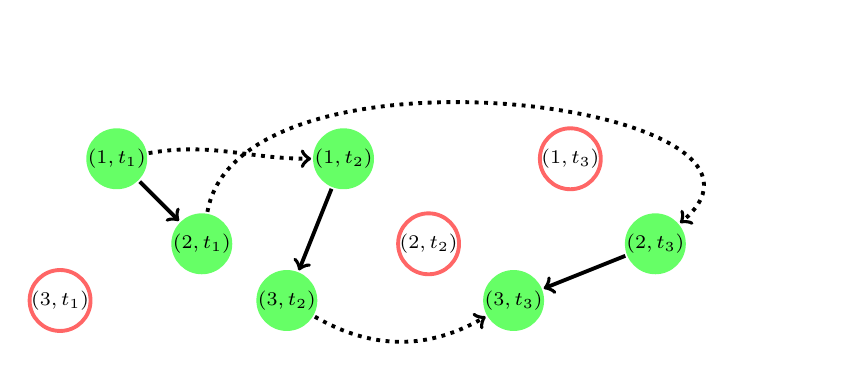
\begin{tikzpicture}[scale=.36, line width =1.4pt]
  \node[circle,fill=green1, minimum size=0.1cm, inner sep = 0pt] (n7) at (-5,7)
{\scriptsize $(2,t_1)$};
  \node[circle,draw=red1, minimum size=0.2cm, inner sep = 0pt] (n8) at (-10,5)
{\scriptsize $(3,t_1)$};
  \node[circle,fill=green1, minimum size=0.1cm, inner sep = 0pt] (n10) at (-8,10) {\scriptsize $(1,t_1)$};

  \node[circle,draw=red1, minimum size=0.2cm, inner sep = 0pt] (n6) at (3,7)
{\scriptsize $(2,t_2)$};
  \node[circle,fill=green1, minimum size=0.2cm,  inner sep = 0pt] (n4) at (-2,5)
{\scriptsize $(3,t_2)$};
  \node[circle,fill=green1, minimum size=0.2cm,  inner sep = 0pt] (n1) at (0,10)
{\scriptsize $(1,t_2)$};

   \node[circle,fill=green1, minimum size=0.2cm,  inner sep = 0pt] (n11) at (11,7)
{\scriptsize $(2,t_3)$};
  \node[circle,fill=green1, minimum size=0.2cm,  inner sep = 0pt] (n12) at (6,5)
{\scriptsize $(3,t_3)$};
  \node[circle,draw=red1, minimum size=0.2cm,  inner sep = 0pt] (n14) at (8,10)
{\scriptsize $(1,t_3)$};

  \foreach \from/\to in {n10/n7, n1/n4, n11/n12}
   \draw[every edge,->] (\from) -- (\to);
     \draw[dotted,->](n7) to[out=80, in=40] (n11);
  \draw[dotted,->](n10) to[out=10, in=180] (n1);
   \draw[dotted,->](n4) to[out=-30,in=-150] (n12);
    \end{tikzpicture}
\end{center}
\caption{A static graph corresponding to the evolving graph example of
Figure~\ref{fig:eg_shortest_walk}. The green nodes are active nodes while the
red nodes are inactive nodes.
The black lines are edges in the static edge set $\tilde E$ and are encoded
algebraically in the diagonal blocks $A^{[t]}$ of the adjacency matrix $\bm M_3$.
The dotted lines are edges in the causal edge set $E'$ and are encoded algebraically in
the off-diagonal blocks $M^{[t_i, t_j]}$.
The graph containing all the edges and temporal nodes has adjacency matrix $\bm M_3$.}
\label{fig:static}
\end{figure}


We derive the block google matrix as a combination of block matrix $A$ and its transpose $A^T$.

The block google matrix is defined as

\begin{lstlisting}
function block_google_matrix(g::IntAdjacencyList; alpha = 0.85, balance = 0.75)
  A = full(block_adjacency_matrix(g))
  A = balance * A + (1-balance) * A'
  N, N = size(A)
  p = ones(N)/N
  dangling_weights = p
  dangling_nodes = find(x->x==0, sum(A,2))

  for node in dangling_nodes
      A[node,:] = dangling_weights
  end
  A ./= sum(A,2)
  return alpha * A .+ (1- alpha) * p
end
\end{lstlisting}

We find the ranking for Figure \ref{}

\begin{lstlisting}
9-element Array{Complex{Float64},1}:
 0.12278
0.254264
0.0533627
 0.36275
0.350713
0.406792
0.0533627
0.524112
0.468848
\end{lstlisting}

One potential problem is the computational cost. Since the dimension of the block matrix
is $|V| \times |T|$, where $|V|$ represents the number of nodes and $|T|$ represents the number of time stamps. The block matrix may become very large for an evolving graph with many time stamps.

\section{Experiments}
\label{sec:experiments}

We test the influence of time on evolvign graph centralities.

\subsection{Random Evolving Graphs}
\label{sec:random}

Note the random evolving graphs are conducted using \texttt{IntAdjacencyList}, which gives better performance for
forward\_neighbors.

We generate a random evolving graph with $100$ nodes and $9771$ static edges and $5$ time stamps.
Here are the top $10$ nodes we find using the Katz Centrality

Since we only are interested in the top nodes.

\begin{tabular}{ l | c }
  \hline
  node & score \\
  334 & 0.152288 \\
  9 & 0.137403 \\
  428 & 0.126793 \\
  164 & 0.121582 \\
  250 & 0.117862 \\
  35 & 0.117627 \\
  291 & 0.105793 \\
  414 & 0.0975953 \\
  123 & 0.096394 \\
  478 & 0.0945754 \\
  \hline
\end{tabular}



We find identify the top $10$

We test temporal Katz centrality,  for top $20$
temporal closeness, and temporal pagerank.
by varing the influence of temporal distance.



Katz score | temporal katz at with time influence 0.1 | temporal katz with time influence 1.0


Closeness with time influence 0.1 | closeness with time influence 1.0


PageRank with time influence 0.1 | PageRank with time influence 1.0



\subsection{JMLR Coauthor Network}
\label{sec:jmlr-coauth-netw}

We construct the evolving coauthor network from Etymo (\url{https://etymo.io}).
We collected $1566$ publications published by Journal of Machine Learning Research (JMLR) from $2001$ to $2017$ with authors involved. We regard each year
as a time stamp and there are $17$ time stamps in total. At each time stamp, we
create a undirected edge (or two directed edges) between two authors if they have coauthored at least one paper.

Some experiments as above.

Katz score | temporal katz at with time influence 0.1 | temporal katz with time influence 1.0


Closeness with time influence 0.1 | closeness with time influence 1.0


PageRank with time influence 0.1 | PageRank with time influence 1.0



\section{Conclusion}
\label{sec:conclusion}

We describe in details the generalizartion of centrality algorithms for evolving graphs.
We introduce the generalization of PageRank centrality.

\bibliographystyle{plain}
\bibliography{sigproc}

\end{document}

%%% Local Variables:
%%% mode: latex
%%% TeX-master: t
%%% End:
